\documentclass[11pt]{article}
\title{A Fixture Study of Policy-First Campus AI Routing}
\date{}
\author{SIGMA AI-assisted research synthesis}
\usepackage[T1]{fontenc}
\usepackage[utf8]{inputenc}
\usepackage[margin=1in]{geometry}
\usepackage{amsmath,amssymb,booktabs,longtable}
\usepackage{microtype}
\usepackage{titlesec}
\usepackage{tikz}
\usetikzlibrary{fit}
\emergencystretch=2em
\raggedbottom
\linespread{1.07}
\usepackage{xcolor}
\definecolor{blue}{HTML}{24485E}
\titleformat{\section}{\Large\bfseries\sffamily\color{blue}}{\thesection}{0.8em}{}
\titleformat{\subsection}{\large\bfseries\sffamily}{\thesubsection}{0.7em}{}
\setlength{\parskip}{.6em}
\setlength{\parindent}{0pt}
\begin{document}
\maketitle
\begin{center}\small\textit{AI-generated research synthesis \textperiodcentered{} SIGMA}\end{center}

\begin{abstract}
This deterministic engineering fixture uses only the sample project objective to exercise SIGMA paper rendering. It contains no independently conducted investigation, workload measurement, university policy finding, or provider-price analysis. The figure is an illustrative proposal and does not describe an implemented MindRouter federation.
\end{abstract}
\section*{About this paper}
This paper was generated by SIGMA, an AI-assisted research system, from the project's recorded investigations, findings, and supporting evidence.
The analysis and conclusions reflect an automated synthesis of that research. Although SIGMA incorporates evidence tracking, critical review, and consistency checks, the resulting paper has not necessarily undergone independent verification or peer review.
Readers should evaluate its arguments, supporting evidence, and stated limitations before relying on its conclusions.
Research style: Match the genre to the available evidence and clearly distinguish findings, hypotheses, negative results and unresolved questions.
\textit{Claims discussed: }C1
\section{Problem framing}
Universities may compare campus-local, approved frontier, hybrid and cooperative service models under sovereignty and budget constraints. This restates the sample question and is not an empirical finding.

\textit{Claims discussed: }C1
\section{Methods and evidence}
A mocked author response was validated and compiled by SIGMA with Tectonic. No live provider was contacted.

\textit{Claims discussed: }C1
\begin{figure}[htbp]
\centering
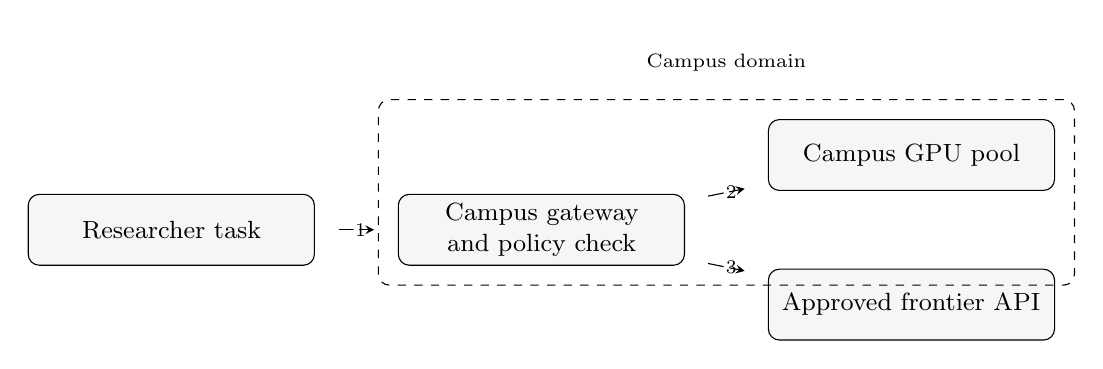
\begin{tikzpicture}[>=stealth, every node/.style={draw, rounded corners, align=center, text width=3.4cm, minimum height=0.9cm, font=\small, fill=blue!5}]
\node (researcher) at (0.0,0.0) {Researcher task};
\node (campus) at (4.7,0.0) {Campus gateway and policy check};
\node (local) at (9.4,0.95) {Campus GPU pool};
\node (frontier) at (9.4,-0.95) {Approved frontier API};
\draw[->,shorten <=3mm,shorten >=3mm] (researcher) -- node[midway,fill=white,draw=none,font=\scriptsize,text width=0pt,minimum height=0pt,inner sep=1pt] {1} (campus);
\draw[->,shorten <=3mm,shorten >=3mm] (campus) -- node[midway,fill=white,draw=none,font=\scriptsize,text width=0pt,minimum height=0pt,inner sep=1pt] {2} (local);
\draw[->,shorten <=3mm,shorten >=3mm] (campus) -- node[midway,fill=white,draw=none,font=\scriptsize,text width=0pt,minimum height=0pt,inner sep=1pt] {3} (frontier);
\node[draw,dashed,rounded corners,inner sep=7pt,fit=(campus)(local),fill=none,label={[font=\scriptsize]above:{Campus domain}}] {};
\end{tikzpicture}
\par\smallskip{\footnotesize 1: request; 2: local eligible; 3: approved only}\
\caption{Illustrative proposal only: campus policy gates any approved external route. This is not an implemented MindRouter federation.}
\end{figure}
\section{Fixture scope}
This fixture tests a safe policy-first routing illustration; it makes no empirical claims about cost, performance, governance or federation.

\textit{Claims discussed: }C1
\section{Interpretation}
The policy gate precedes any proposed external route. This diagram is a rendering test, not an architecture evaluation.

\textit{Claims discussed: }C1
\section{Findings and interpretation}
\subsection{C1 -- Established}
The saved project contains a research objective.
The objective is explicitly present in the project snapshot.
\textit{Evidence: }project:dc98d234-4b89-43e5-962f-aa0182ce9562
\section{Limitations}
\begin{itemize}
\item No Investigator/Skeptic research session or external sources were saved.
\item The architecture is illustrative and unmeasured.
\end{itemize}
\section{Open obligations}
\begin{itemize}
\item Conduct and save substantive research before evaluating campus costs, quality or governance.
\end{itemize}
\section{Conclusions}
This fixture verifies diagram rendering only; it does not answer the research question.

\textit{Claims discussed: }C1
\section*{Evidence and authorship note}
Snapshot SHA-256: 3dcae814d22543d99e4be11f89c0123f8a29d9c7958ca5147f48b7a187c2142e
Generated by an AI author from the cited saved research snapshot. This document is not independent verification. No external bibliography was added.
\section*{Validation warnings}
\begin{itemize}
\item Deterministic mocked artifact; not independently validated research.
\end{itemize}
\end{document}
